\begin{figure}[t!]
    \centering
    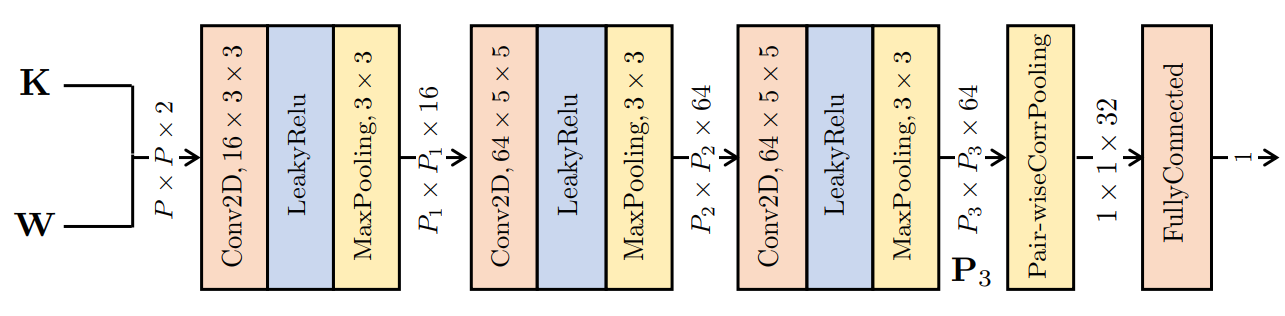
\includegraphics[keepaspectratio, width=0.5\textwidth]{CNN_architecture}
    \caption{Pair-Wise Correlation Network (PCN) architecture}
    \label{fig:CNN_architecture}
\end{figure}

We were assigned the paper \textit{CNN-based fast source device identification} \cite{Mandelli}.

In this paper the authors propose a CNN-based approach to address the problem of source device identification based on PRNU. 
In particular, their goal is to replace the PCE test with an alternative method based on CNN. Their approach differs from \cite{Bondi}
because they train an end-to-end network instead of using a CNN followed by an SVM.

The core idea of this paper is to use a 2-channel CNN to compare the estimated device PRNU $K_d$ with the noise residual $W$ 
obtained from the given test image $I$.

First of all they estimate the device PRNU\cite{Lukas} $K_d$ from a set of flat-field images taken from the same device and they extract the
noise residual $W$ from a set of images depicting natural scenes.
Then they crop the central $P$x$P$ pixel region from both $K_d$ and $W$ and they feed the CNN with these 2 image patches.
Since the method is independent from the used CNN they experiment different pre-trained networks and they propose a simple but 
effective architecture that is composed of 3 convolutional layers, a pair-wise correlation pooling layer and a fully connected 
layer (Fig. \ref{fig:CNN_architecture}). The pair-wise correlation pooling layer computes the correlation between adjacent pairs of features, while the
fully connected layer outputs an identification score $C_s$ that is high for coherent pairs and low for non-coherent ones. 

The network can be used in both a closed-set scenario and in an open-set scenario. In the closed-set scenario we have a finite set 
of devices and we have to identify the source of the image from that set. In the open-set scenario we have a test image and a candidate
device and we have to tell if that device shot the given image.

The authors shows that in both the open and closed set scenario the proposed approach outperforms the PCE test both in accuracy 
and inference time. In particular, regarding the closed set scenario, we can see from Fig. \ref{fig:Closed_set_test} 
that the proposed Pair-wise Correlation Net (PCN) is faster than all the 
other architectures and it outperforms PCE in accuracy, however it is outperformed by the other networks. It is important to notice 
also that all the methods perform better when the patch size is bigger.
Regarding the open set scenario, the area under the ROC curve related to the patch size is shown in Fig. \ref{fig:Open_set_test}  and it's clear that 
PCE is worst than all the proposed architectures. 
Finally, in Fig. \ref{fig:Double_JPEG_compression}, we can see the accuracy as a function of crop size when the dataset is double-JPEG compressed. 
The PCN outperforms PCE even after double compression and we can notice that the performances are better when the network is trained on 
data where the noise residual is extracted from double compressed images.

\begin{figure}[t!]
    \centering
    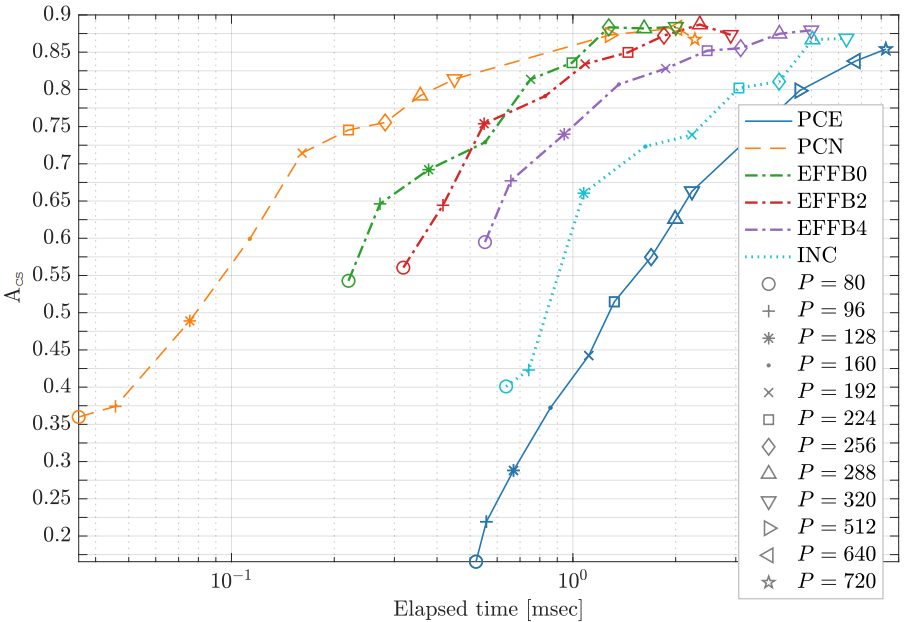
\includegraphics[keepaspectratio, width=0.5\textwidth]{Closed_set_test}
    \caption{Accuracy $A_cs$ as a function of time [milliseconds] and crop size $P$.}
    \label{fig:Closed_set_test}
\end{figure}

\begin{figure}[t!]
    \centering
    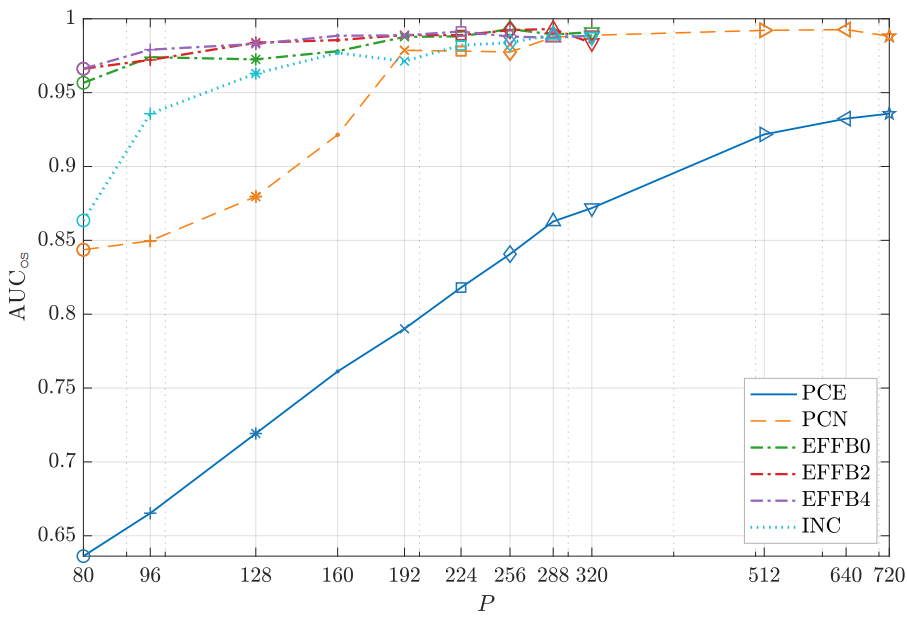
\includegraphics[keepaspectratio, width=0.5\textwidth]{Open_set_test}
    \caption{Area under the ROC curve $AUC_os$ as a function of crop size $P$.}
    \label{fig:Open_set_test}
\end{figure}

\begin{figure}[t!]
    \centering
    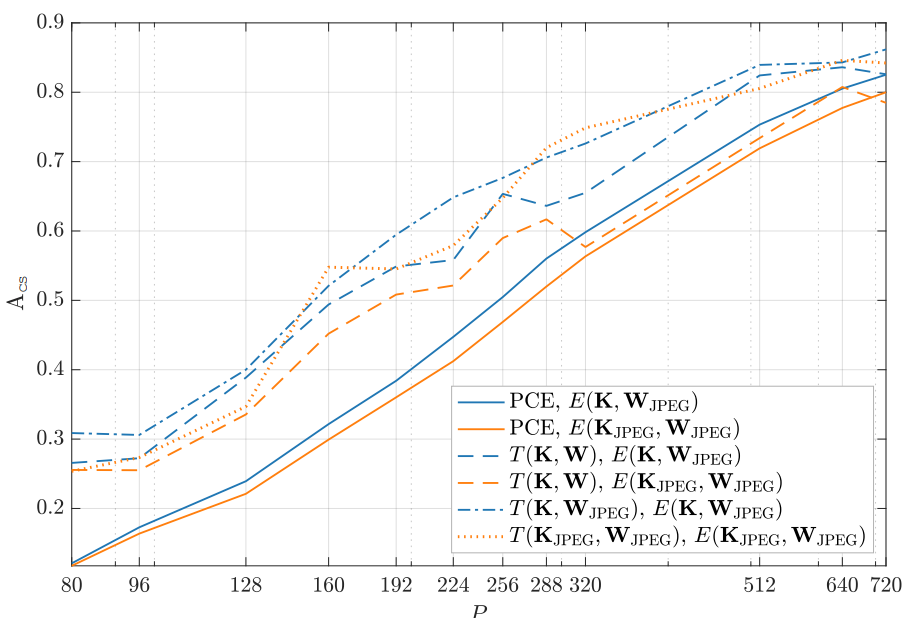
\includegraphics[keepaspectratio, width=0.5\textwidth]{Double_JPEG_compression}
    \caption{Accuracy $A_cs$ as a function of crop size $P$, considering double-JPEG
    compressed dataset with quality 90 and PCN network. $T(·)$ and $E(·)$ refer
    to training and evaluation datasets, respectively.}
    \label{fig:Double_JPEG_compression}
\end{figure}